\section{Discussion and Future Work}
\label{sec:discussion}
In this section, we answer our research questions and discuss our interpretation of this result. We then highlight recommendations to practitioners using QS for collective decision making and highlight future directions for QS research.

\subsection{QS's effectiveness and its dual components}
In this study, we aim to examines how effectively QS captures participant preferences compared to Likert scale surveys at a pairwise level (RQ1) and understand whether QS requires both the quadratic cost function and a fixed budget to make it effective (RQ2). Our dual analysis comparing QS (votes and credit spent), Likert, UQS, and LS further supports that QS exhibits superior performance in preference elicitation compared to Likert Scale Surveys. Within ordinal preference prediction, QS shows a statistically significant but modest advantage over Likert scales, even QS with small budget. For preference intensity, QS performs better Likert scale surveys as the magnitude of preference differentials increases between options. Altogether, we demonstrated that QS better Likert overall should the survey designer aim to capture accurate individual preferences across multiple options under resource constraint scenarios for collective decision making.

With the added experiment in this study, our empirical findings demonstrates both the quadratic cost function and budget constraint constitute the effectiveness of QS mechanism. The removal of either component (as implemented in Unlimited QS or Linear Survey) results in diminished performance as discussed in~\Cref{sec:result_2}. Pragmatically, this result indicates that rather than applying LS for reduced cognitive load and ease of completion, further research should guide developers in designing systems that aids QS completion. Scientifically, the result raised our interest to understand why LS did not work as well.

% insert figure
\begin{figure}[h]
    \centering
    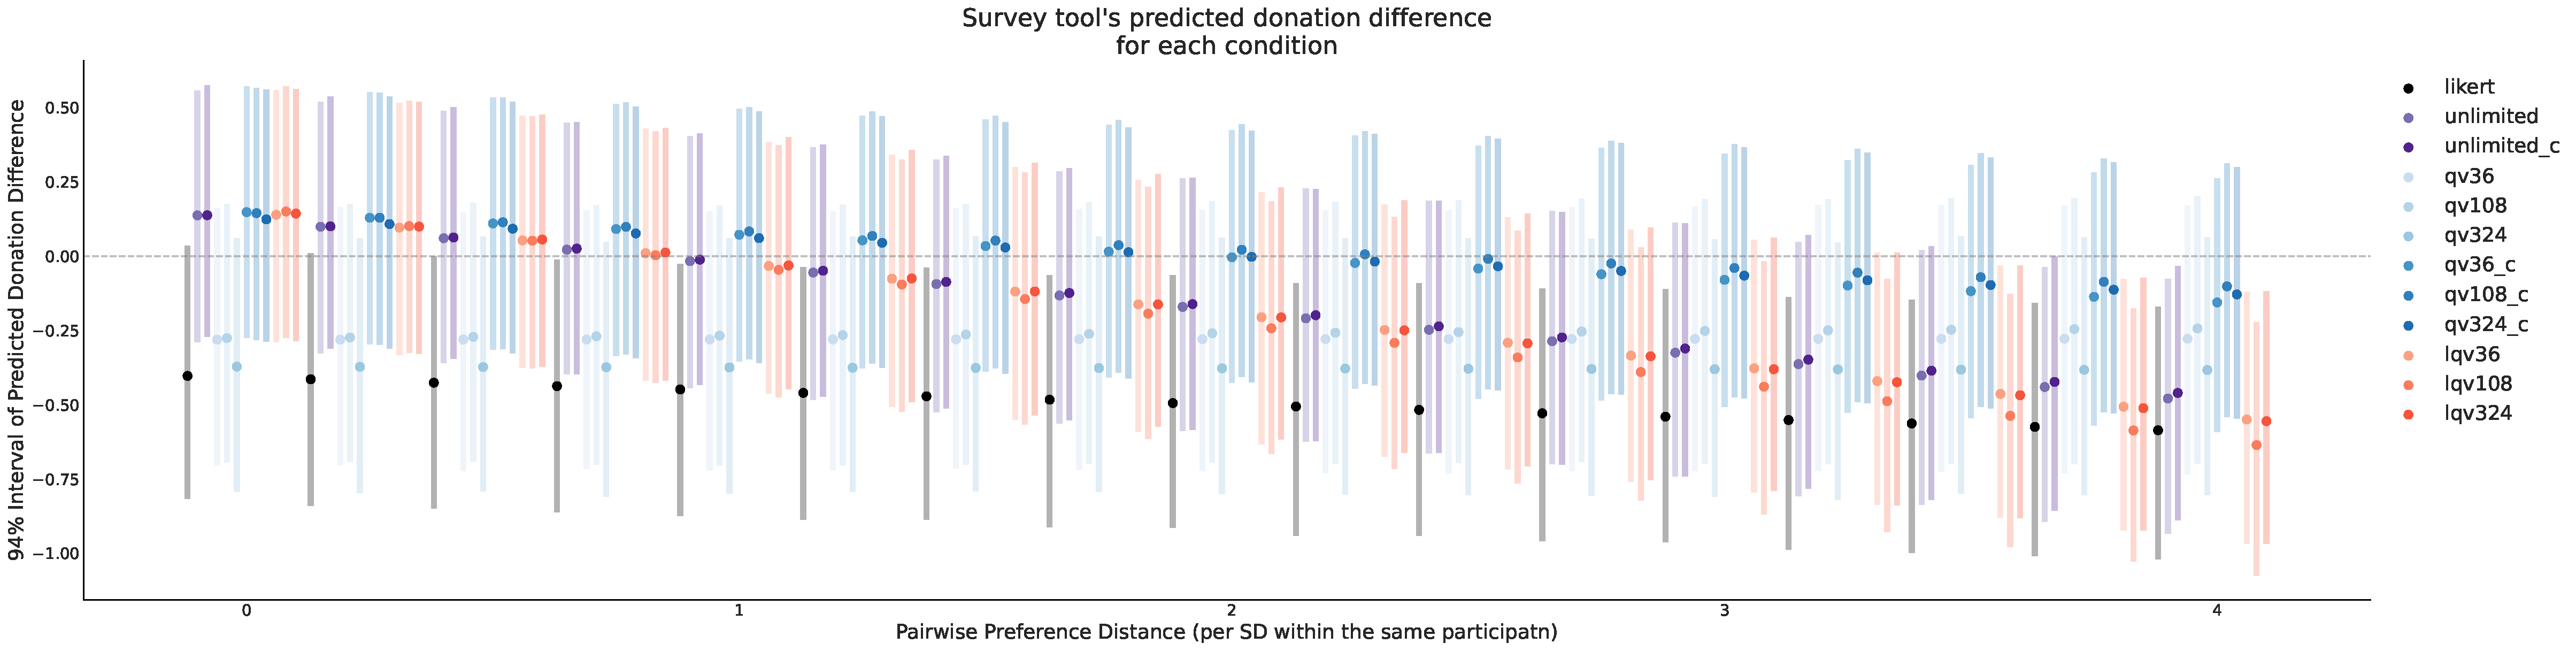
\includegraphics[width=\textwidth]{content/image/Predicted_Donation_Diff_Interval.pdf}
    \caption{Comparison of preference elicitation methods: QS, LS, UQS, and Linear Survey.}
    \label{fig:comparison}
\end{figure}


\subsection{Distortion in survey's `preference units'}
The goal of QS aims to identify nuances among multiple options, which reflected the aim to elicit quantified differences between options. Among options, preference differences lies strong between some pairs and less among others. As discussed in~\Cref{sec:interval_measures}, QS credits and votes remain reflective of individual's behavior regardless of preference strength.~\Cref{fig:comparison} plots how well different tools predict participant behaviors as preference differences increases. LS, regardless of credit size, reflects that the stronger a participant treat a pairwise option across all options, the more LS response underestimates this preference.

Two plausible explanations lies in distortion in how individuals percieve each additional `unit preference,' which we define as the additional preference interval the participant expressed (i.e., an additional vote, or selecting the next preference interval). The first can be a participants expericing simple diminishing returns~\cite{mankiwPrinciplesEconomics2018} like in economics, for which when adding votes, participants would add less than the amount as they felt that additional votes creates diminishing returns, hence the underestimation. 

Another explaination echos the Weber-Fechner law~\cite{}. The former states that the `just noticeable difference' between two stimuli is proportional to the baseline intensity of the stimulus. And the latter states that the percieved intensity of a stimulus grows logarithmically. What we observed here is that participants responding to LS exhibited less `percieved' preference per unit as the preference difference increases between two options. This percieved difference adds up to create the illusion that the survey participant had expressed enough votes as their presented preference. Early CSS validating by~\citet{dudekValidityPointAssignmentProcedure1957} cautions that participants may not recognize the nonlinear relationship between point-assignment, leading them to misjudge how much their numerical input actually reflects their intended intensity. Conversely, QS forces each additional vote cost to grow quadratically. This approach seems to corrected the underestimation since each additional `preference unit' is more costly, correcting the percieved preferences individuals experienced.

Since QS credits and votes are inter-related, we believe that this correction in distortion helped QS votes to reflect resonablly well the presented preferences of the individual, albiet the credits performs slightly better without statistical differences as shown in Figure X.

\subsection{Choice overload on survey options}
In terms of ordinal difference, with think that the total budget creating too many options is a plausible explaination of why LS and UQS underperforms Likert and QS.

The total budget serves two purposes. Other than setting the unit simulus we discussed in the previous subsection, the total budget also limits the number of plausible selections for each survey option. Thus, LS18 means that a participant can consider 18 plausible selections for each option, equivalent to QS324. This number of choices increases drastically as the LS credits increases.

The quadratic cost drastically reduces participant's decision space as they began allocating votes since the votes come at a quadratic cost. LS's linear cost maintained hightened vote options as participants complete the task. This increase in option likey introduced choice overload that nudged individual's to express satisficing behaviors~\cite{}. Thus, we see deteriorting ordinal behaviors in LS as credits increase.

This abundance of credits in LS reflected by UQS credit usages, which we found a long tail of udage with half of the participants stop answering the survey after sprending 45 credits. This value reflects when a participants think that they have enough expression power to the options presented to them.

Likert's 5-point scale likey limited participant's preference expression ability as the prior study discusses~\cite{chengCanShowWhat2021}.

The complementary effects of preference distortion and choice overload might explain why both QS components are necessary. The quadratic cost function corrects for the perceptual distortion in how participants express preference intensity, addressing the underestimation that occurs with linear scales as preference differences grow larger. Meanwhile, the budget constraint reduces the decision space, mitigating choice overload that leads to satisficing behaviors.  Together, these mechanisms create a survey instrument that better refelcts survey participant's responses comapred to their behaviors.


\subsection{Takeaway for practitioners}
Our findings offer several practical implications for practitioners employing preference elicitation methods. When selecting survey instruments, researchers should first clearly identify their measurement objectives. For simple individual preference rankings where intensity is not critical, Likert scales may provide adequate performance with greater simplicity, though our results indicate QS still offers modestly better alignment with revealed preferences. However, when measuring collective preferences that require aggregating varying preference intensities, QS significantly outperforms traditional methods, particularly in capturing strong preference differentials that Likert scales systematically underestimate. Both components of QS—the quadratic cost function and budget constraint—are essential for accurate preference elicitation, as removing either component (as in UQS or LS) substantially reduces performance. While different budget allocations show minimal differences in outcomes, our analysis suggests that a budget of 36 credits offers optimal stability from a Bayesian perspective, providing sufficient expressiveness without introducing unnecessary complexity.

\section{Limitations and Future work}
\label{sec:limitations}

\paragraph{`True preferences' and survey instruments}
It is important to acknowledge limitations in our approach to measuring "true preferences." While donation behaviors aim to mirror tangible, monetary contributions with real stakes creating incentive compatibility, not all preferences are naturally expressed through monetary means. External factors such as prior charitable giving, personal connections to causes, or tax implications might influence donation decisions independent of underlying preference structures.

\paragraph{Charities and government resource allocation}
Our experimental design using charitable donations as a proxy for preference intensity may not fully capture the dynamics of government resource allocation decisions. Charitable giving operates under different incentive structures and social contexts compared to public resource allocation. Government spending decisions typically involve complex political considerations, longer-term consequences, and different accountability mechanisms that our experiment cannot fully simulate. Future research could examine QS applications in field studies of actual resource allocation decisions.

\paragraph{Future Work: mental model construction of QS respondents}
This paper layed the ground for future research to conduct interview and construct mental models to better understand how one constructs and balance between perceived preferences (internal valuation) and presented preferences (expressed through the survey mechanism). Our results suggest that QS helps correct distortions in how people express preference intensity, but the precise cognitive mechanisms remain unclear. Prior literature has highlighted this gap but cognitive interviews could elucidate how participants interpret and navigate the quadratic cost structure.

\paragraph{Future Work: comparing QS with other forced-choice methods}
LS's less effective outcome makes future comparative analysis between QS and other forced-choice preference elicitation tools such as Knapsack Surveys (KS) and conjoint analysis important. Each method employs different constraints and mechanisms to reveal preference intensity. Understanding how these methods perform across various decision contexts and preference distributions would help practitioners select appropriate tools for specific applications. Future research should focus on 

Such comparisons should examine not only elicitation accuracy but also user experience, cognitive load, and susceptibility to strategic manipulation.






% \subsection{Votes in QS are designed for aggregation}
% Emperically, we see 


% # Relationships Between Linear Voting, Donation Behavior, Budget in Quadratic Surveys, and Quadratic Survey Votes

% ## 1. Linear Voting
% - **Concept**: In linear voting systems, each vote is treated equally, and the cost of each additional vote remains constant.
% - **Outcome**: The difference in vote counts between options directly translates to perceived preference, assuming linear preference increments.
% - **Limitation**: It may not accurately reflect strong intensity differences, as stronger preferences are not weighted differently.

% ## 2. 

% ## 3. Budget in Quadratic Surveys
% - **Concept**: Participants have a limited budget to allocate votes, with costs increasing quadratically.
% - **Outcome**: Forces participants to weigh their choices more carefully, making stronger preferences more costly to express.
% - **Advantage**: Better reflects the strength of preferences as each additional vote requires more effort (cost).
% - **Limitation**: Interpretation of budgets requires understanding the quadratic nature and its impact on expressed preferences.

% ## 4. Quadratic Survey Votes
% - **Concept**: Uses a quadratic cost structure to allocate votes, where each additional vote costs more.
% - **Outcome**: Encapsulates stronger preferences through higher costs, making it harder for majority preferences to dominate without significant effort.
% - **Advantage**: Mitigates tyranny of the majority by making it costlier to exert higher influence.
% - **Interpretation**: The aggregate votes reflect group preferences, but do not linearly correspond to preference strength.

% ## Conclusion
% Understanding these relationships provides a comprehensive view of how different voting mechanisms capture preference intensity.
